
\documentclass[openany,11pt]{homework}

\coursename{ELEN 4903 Machine Learning (Spring 2018)} % DON'T CHANGE THIS

\studname{Pratyus Pati}    % YOUR NAME GOES HERE
\studmail{pp2636@columbia.edu}% YOUR UNI GOES HERE
\hwNo{1}                   % THE HOMEWORK NUMBER GOES HERE

% Uncomment the next line if you want to use \includegraphics.
\usepackage{graphicx}

\begin{document}
\maketitle

\section*{Problem 1(a)}

Given:
\begin{equation}
x_i \in \{0, 1\}
\end{equation}
Every random variable is taken from a Bernoulli's distribution
\begin{equation}
p(x_i\mid\pi) = \pi^{x_i}(1-\pi)^{1-x_i}, \pi \in [0, 1]
\end{equation}
To find:\\
Joint distribution of the data:
$$
p(x_1, x_2, ..., x_n \mid \pi)
$$
Since each random variable is I.I.D,
\begin{align}
	p(x_1, x_2, ..., x_n \mid \pi) & = \prod_{i = 1}^{n} p(x_i \mid \pi) \\
								   & = \prod_{i = 1}^{n} \pi^{x_i}(1-\pi)^{1-x_i} \\
								   & = \pi^{\sum_{i=1}^{n} x_i}(1-\pi)^{(n-\sum_{i=1}^{n} x_i)}
\end{align}
Let $\mu = (\sum_{i=1}^{n} x_i)/ n$ In which case, \\
$$
p(x_1, x_2, ..., x_n \mid \pi) = \pi^{n\mu}(1-\pi)^{n-n\mu}
$$

\section*{Problem 1(b)}

\begin{align}
\hat{\pi}_{ML} & = \operatornamewithlimits{arg\,max}_{\pi} p(x_1, x_2, ..., x_n \mid \pi) \\
			   & = \operatornamewithlimits{arg\,max}_{\pi} \pi^{n\mu}(1-\pi)^{n-n\mu} \\
			   & = \operatornamewithlimits{arg\,max}_{\pi} \ln(\pi^{n\mu}(1-\pi)^{n-n\mu}) \\
			   & = \operatornamewithlimits{arg\,max}_{\pi} [(n\mu) (\ln \pi)] + [(n - n\mu)(\ln (1-\pi))]
\end{align}

On taking the derivative w.r.t. $\pi$\\
\begin{align}
\frac{\partial }{\partial \pi} [(n\mu) (\ln \pi)] + [(n - n\mu)(\ln (1-\pi))]
& = \left[n\mu \frac{\partial \ln \pi}{\partial \pi}\right] + \left[(n - n\mu)\left(\frac{\partial \ln(1-\pi)}{\partial \pi}\right)\right] \\
& = \frac{n\mu}{\pi} -\frac{n-n\mu}{1-\pi}
\end{align}

On setting the partial derivative w.r.t $\pi$ as 0 to get $\hat{\pi}_{ML}$,
\begin{align}
\frac{n\mu}{\hat{\pi}_{ML}} -\frac{n-n\mu}{1-\hat{\pi}_{ML}} & = 0 \\
\Rightarrow n\mu(1-\hat{\pi}_{ML}) - (n-n\mu)(\hat{\pi}_{ML}) & = 0 \\
\Rightarrow n\mu - n\mu\hat{\pi}_{ML} - n\hat{\pi}_{ML} + n\mu\hat{\pi}_{ML} & = 0 \\
\Rightarrow n\mu - n\hat{\pi}_{ML} & = 0 \\
\Rightarrow \hat{\pi}_{ML} & = \mu = \frac{\sum_{i=1}^{n} x_i}{n}
\end{align}

\section*{Problem 1(c)}

\[
p(\pi) = beta(a, b) = \frac{\pi^{a-1}(1-\pi)^{b-1}}{B(a, b)}
\]

\begin{align}
p(\pi \mid x_1, x_2, ..., x_n) & = \frac{p(x_1, x_2, ..., x_n \mid \pi)p(\pi)}{p(x_1, x_2, ..., x_n)} \\
							   & = \frac{\pi^{n\mu}(1-\pi)^{n-n\mu}\pi^{a-1}(1-\pi)^{b-1}}{B(a, b)p(x_1, x_2, ..., x_n)} \\
							   & = \frac{\pi^{n\mu+a-1}(1-\pi)^{n-n\mu+b-1}}{B(a, b)p(x_1, x_2, ..., x_n)}
\end{align}

\begin{align}
\hat{\pi}_{MAP} & = \operatornamewithlimits{arg\,max}_{\pi} p(\pi \mid x_1, x_2, ..., x_n) \\
& = \operatornamewithlimits{arg\,max}_{\pi} \frac{\pi^{n\mu+a-1}(1-\pi)^{n-n\mu+b-1}}{B(a, b)p(x_1, x_2, ..., x_n)} \\
& = \operatornamewithlimits{arg\,max}_{\pi} \left[\pi^{n\mu+a-1}(1-\pi)^{n-n\mu+b-1}\right] \\
& = \operatornamewithlimits{arg\,max}_{\pi} \left[\ln(\pi^{n\mu+a-1}(1-\pi)^{n-n\mu+b-1})\right]	\\
& = \operatornamewithlimits{arg\,max}_{\pi} \left[(n\mu+a-1)\ln\pi + (n-n\mu+b-1)\ln(1-\pi)\right] \\
\end{align}

On taking the derivative w.r.t. $\pi$
\begin{align}
& \frac{\partial }{\partial \pi} \left[(n\mu+a-1)\ln\pi + (n-n\mu+b-1)\ln(1-\pi)\right] \\
= & \left[(n\mu+a-1) \frac{\partial \ln \pi}{\partial \pi}\right] + \left[(n-n\mu+b-1)\left(\frac{\partial \ln(1-\pi)}{\partial \pi}\right)\right] \\
& = \frac{n\mu+a-1}{\pi} -\frac{n-n\mu+b-1}{1-\pi}
\end{align}

On setting the partial derivative w.r.t $\pi$ as 0 to get $\hat{\pi}_{MAP}$,
\begin{align}
\frac{n\mu+a-1}{\hat{\pi}_{MAP}} -\frac{n-n\mu+b-1}{1-\hat{\pi}_{MAP}} & = 0 \\
\Rightarrow (n\mu+a-1)(1-\hat{\pi}_{MAP}) - (n-n\mu+b-1)(\hat{\pi}_{MAP}) & = 0 \\
\Rightarrow (n\mu + a - 1) - (n\mu + a - 1 + n - n\mu + b - 1)\hat{\pi}_{MAP} & = 0 \\
\Rightarrow (n\mu + a - 1) - (n + a + b - 2)\hat{\pi}_{MAP} & = 0 \\
\Rightarrow \hat{\pi}_{MAP} & = \frac{n\mu + a - 1}{n + a + b - 2} \\
							& = \frac{n\sum_{i=1}^{n} x_i + a - 1}{n + a + b - 2}
\end{align}

\section*{Problem 1(d)}

\begin{align}
p(\pi \mid x_1, x_2, ..., x_n) & = \frac{p(x_1, x_2, ..., x_n \mid \pi)p(\pi)}{p(x_1, x_2, ..., x_n)} \\
& = \frac{\pi^{n\mu}(1-\pi)^{n-n\mu}\pi^{a-1}(1-\pi)^{b-1}}{B(a, b)p(x_1, x_2, ..., x_n)} \\
& = \frac{\pi^{n\mu+a-1}(1-\pi)^{n-n\mu+b-1}}{B(a, b)p(x_1, x_2, ..., x_n)} \\
& \propto \pi^{n\mu+a-1}(1-\pi)^{n-n\mu+b-1}				\\
\end{align}

Therefore, the posterior probability is proportional to the $beta$ distribution. We can convert the proportionality to an equality by adding the correct co-efficient to form the $beta$ distribution

\begin{align}
p(\pi \mid x_1, x_2, ..., x_n) & \propto \pi^{n\mu+a-1}(1-\pi)^{n-n\mu+b-1}\\
& = \frac{\pi^{n\mu+a-1}(1-\pi)^{n-n\mu+b-1}}{B(a + n\mu, b + n-n\mu)} \\
& = beta(a + n\mu, b + n-n\mu)
\end{align}

\section*{Problem 1(e)}
The mean of the distribution $beta(a, b)$ is given by $\frac{a}{a+b}$ \\
Therefore, \\
\begin{align}
\mathbb{E}[\pi_{post}] & = \frac{a + n\mu}{b + n - n\mu + a + n\mu} \\
				& = \frac{a + n\mu}{a + b + n} \\
				& = \frac{a}{a+b+n} + \mu\frac{n}{a+b+n} \\
				& = \frac{a}{a+b}\frac{a+b}{a+b+n} + \mu\frac{n}{a+b+n} \\
\end{align}
This can be represented as:
\begin{align}
\mathbb{E}[\pi_{post}] & = \alpha\mathbb{E}[\pi_{prior}] + (1-\alpha)\hat{\pi}_{ML}
\end{align}
This proves that $\mathbb{E}[\pi_{post}]$ is a weighted average of $\mathbb{E}[\pi_{prior}]$ and $\hat{\pi}_{ML}$,where $\alpha = \frac{a+b}{a+b+n}$ that tends to 0 as n increases. Therefore, we can say:
\begin{align}
\lim_{n\to\infty}\mathbb{E}[\pi_{post}] & = \hat{\pi}_{ML}
\end{align}

Also, for relating $\mathbb{E}[\pi_{post}]$ and $\hat{\pi}_{MAP}$,
\begin{align}
	\mathbb{E}[\pi_{post}] & = \frac{a + n\mu}{a+b+n} \\
												 & = \frac{a + n\mu -1+1}{a+b+n} \\
												 & = \frac{a+n\mu-1}{a+b+n} + \frac{1}{a+b+n} \\
												 & = \frac{a+n\mu-1}{a+b+n-2}\frac{a+b+n-2}{a+b+n} + \frac{1}{2}\left(1-\frac{a+b+n-2}{a+b+n}\right)
\end{align}

This can be represented as:
\begin{align}
\mathbb{E}[\pi_{post}] & = \alpha\hat{\pi}_{MAP} + (1-\alpha)(0.5)
\end{align}

This proves that $\mathbb{E}[\pi_{post}]$ lies between $\hat{\pi}_{MAP}$ and $0.5$, and approaches $\hat{\pi}_{MAP}$ as $n \to \infty$.

The variance of the distribution $beta(a, b)$ is given by $\frac{ab}{(a+b)^2(a+b+1)}$ \\
Therefore, \\
\begin{align}
var[\pi_{post}] & = \frac{(a + n\mu)(b + n - n\mu)}{(b + n - n\mu + a + n\mu)^2(b + n - n\mu + a + n\mu +1)} \\
& = \frac{(a + n\mu)(b + n - n\mu)}{(a + b + n)^2(a + b + n+1)}
\end{align}
For relating it with the mean, the variance can be further represented as:
\begin{align}
	var[\pi_{post}] & = \left(\frac{1}{a+b+n+1}\right)\left(\frac{a+n\mu}{a+b+n}\right)\left(1-\frac{a+n\mu}{a+b+n}\right) \\
	& = \left(\frac{1}{a+b+n+1}\right)\left(\mathbb{E}[\pi_{post}]\right)\left(1-\mathbb{E}[\pi_{post}]\right)
\end{align}
From this relation, we can see that $var[\hat{\pi}_{MAP}]$ is a quadratic funtion of $\mathbb{E}[\pi_{post}]$ and exists for the range $\mathbb{E}[\pi_{post}] \in [0, 1]$, 0 at $\mathbb{E}[\pi_{post}] \in \{0, 1\}$ and achieves its maximum at $\mathbb{E}[\pi_{post}] = 0.5$
\\
\\
From the above results, we can see how $var[\pi_{post}]$ varies with respect $\mathbb{E}[\pi_{post}]$ due to changes in $\hat{\pi}_{ML}$ and $\hat{\pi}_{MAP}$. Also, as $n \to \infty$, $\mathbb{E}[\pi_{post}]$, $\hat{\pi}_{MAP}$ and $\hat{\pi}_{ML}$ converge.



\section*{Problem 2(a)}
\begin{figure}[h]
	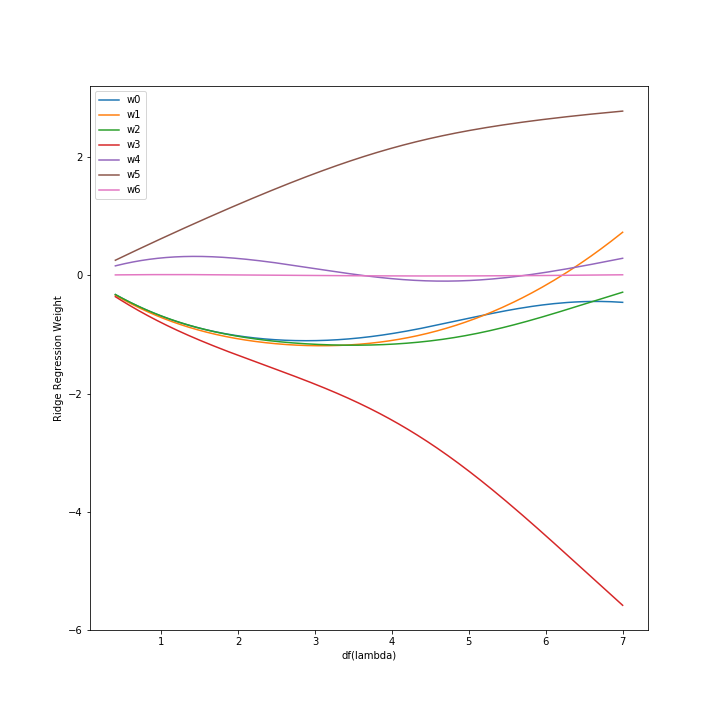
\includegraphics[width=\textwidth]{wrr_vs_dfl}
	\caption{Ridge Regression Weights vs. Degrees of Freedom $df(\lambda)$}
\end{figure}

\section*{Problem 2(b)}
From the figure plotting the relationship between $w_i$ and $df(\lambda)$, it can be seen that there are two coefficients $w_3$ and $w_5$ that exhibit large magnitudes for normal least square condition. On decreasing the degrees of freedom ($df(\lambda)$) by increasing $\lambda$, these coefficients gradually converge towards 0.
\\
\\
These coefficients can either be uncorrelated values whose magnitudes signify their respective importance in calculating the predicted value. $w_5$ is positively correlated with the value of $\hat{y}$, and therefore, $\hat{y}$ increases as the $6^{th}$ feature increases. $w_3$ is negatively correlated with $\hat{y}$, and therefore $\hat{y}$ decreases as $4^{th}$ feature decreases.
\\
\\
Alternatively, $4^{th}$ and $6^{th}$ features are correlated and as a result, $w_{LS}$ is poorely determined, with high variance. Ridge regression helps in decreasing the variance of such weights by restraining it around 0.

\section*{Problem 2(c)}
\begin{figure}[h]
	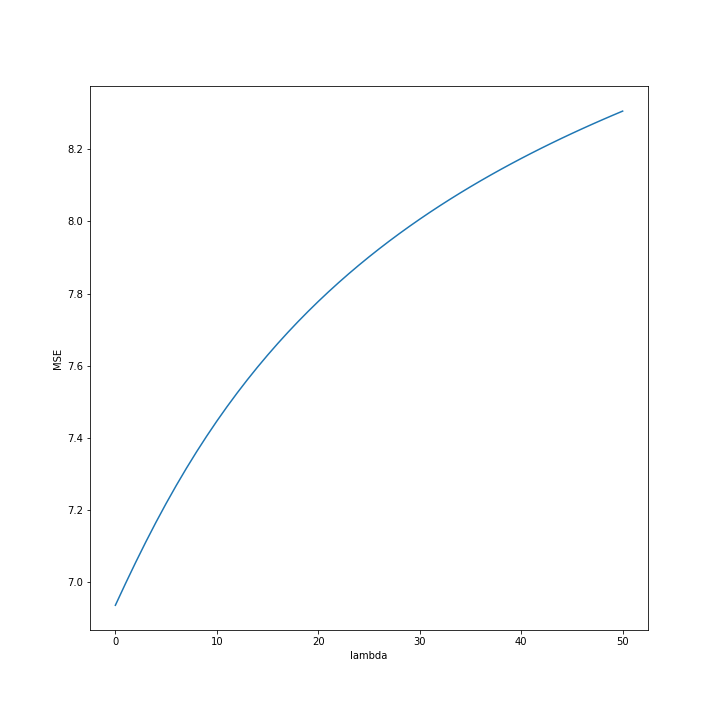
\includegraphics[width=\textwidth]{MSE_vs_lambda}
	\caption{Mean Square Error vs. $\lambda$}
\end{figure}

From the figure, it can be seen that as $\lambda$ increases, the Mean Square Error increases accordingly. In this case, trying to decrease the variance by increasing $\lambda$, introduces too much bias into the model. In such a case, we would like to keep $\lambda$ as low as possible to reduce the bias.

\section*{Problem 2(d)}
\begin{figure}[h]
	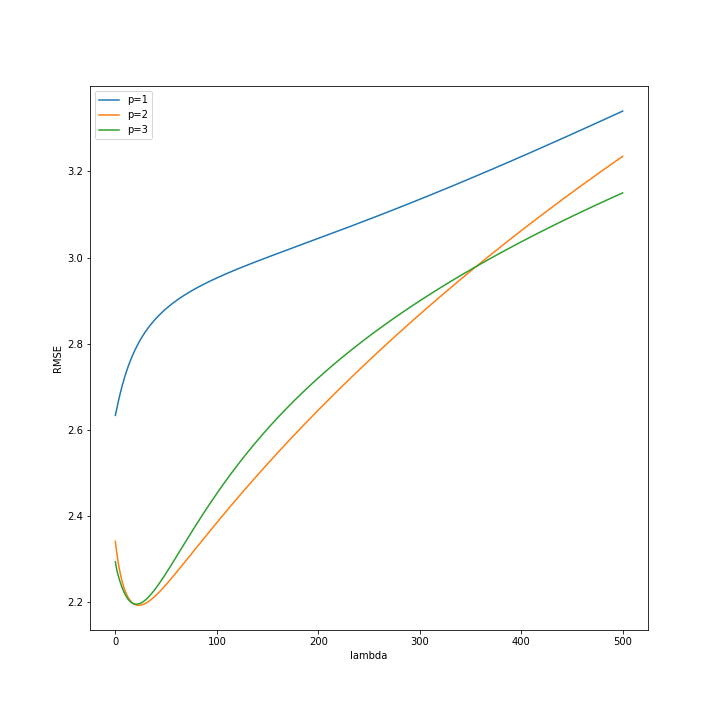
\includegraphics[width=\textwidth]{RMSE_vs_lambda_p}
	\caption{Root Mean Square Error vs. $\lambda$ for differernt values of $p$}
\end{figure}

We can see that as we add more $p^{th}$ order terms, the RMSE decrease. Also for p = 2 and 3, there is a clear local minima of the RMSE with respect to the $\lambda$. Hence, we can set $\lambda$ to the minumum value, and use the Occam's Razor heuristic to select p as 2 to create the simplest possible model that decreases the RMSE.



\end{document}
